\chapter{NMR गहराई में: स्पंद, विश्रांति और द्विविमीय स्पेक्ट्रम}\label{ch:b3:advanced-nmr}

अस्पताल का MRI स्कैनर और रसायन विभाग का NMR स्पेक्ट्रममापी
एक ही सिद्धांत पर कार्य करते हैं। दोनों हाइड्रोजन नाभिकों को एक प्रबल चुंबकीय
क्षेत्र में रखते हैं, रेडियो तरंगों के एक छोटे स्पंद से उनके चुंबकन को झुकाते हैं, और
उस मंद संकेत को सुनते हैं जिसे वह पुरस्सरण और विश्रांति के दौरान प्रेरित करता है।
स्कैनर संकेत को कोमल ऊतक के प्रतिबिंब में बदलता है; स्पेक्ट्रममापी उसे
रासायनिक विस्थापनों और युग्मनों की सूची में, और लगातार कई स्पंदों के साथ ऐसे
द्विविमीय मानचित्रों में जो दिखाते हैं कि कौन-सा परमाणु किससे आबंधित है। यह
अध्याय समझाता है कि स्पंद क्या करते हैं, संकेत क्यों मंद पड़ता है, और
\omterm{def:b3:advanced-nmr:two-d}{द्विविमीय स्पेक्ट्रम} कैसे पढ़े जाते हैं --- वह विधि जिससे आज अधिकांश नई कार्बनिक
संरचनाएँ हल की जाती हैं।

\begin{recall}
प्रथम वर्ष के खंड ने ${}^1$H NMR स्पेक्ट्रमों की व्याख्या की: रासायनिक विस्थापन, परिरक्षण,
तुल्य प्रोटॉन, समाकलन, चक्रण--चक्रण युग्मन, युग्मन स्थिरांक और
बहुक। द्वितीय वर्ष के खंड ने विस्तृत-पट्ट वियुग्मन और DEPT के साथ ${}^{13}$C NMR
जोड़ा, जिसके स्पंद अनुक्रम को उसने दिया हुआ माना था; स्पंदों की व्याख्या यहाँ की गई है।
\Cref{ch:b3:many-electron-atoms} ने चक्रण को एक कोणीय संवेग के रूप में लिया। भौतिकी
से: क्षेत्र में स्थित चुंबकीय आघूर्ण की ऊर्जा $-\boldsymbol\mu\cdot\mathbf B$ है, और
स्तरों की समष्टियाँ बोल्ट्समान गुणक $\eu^{-\Delta E/kT}$ का अनुसरण करती हैं, जिसे
\cref{ch:b3:partition-functions} में विकसित किया गया है।
\end{recall}

\begin{omfigure}
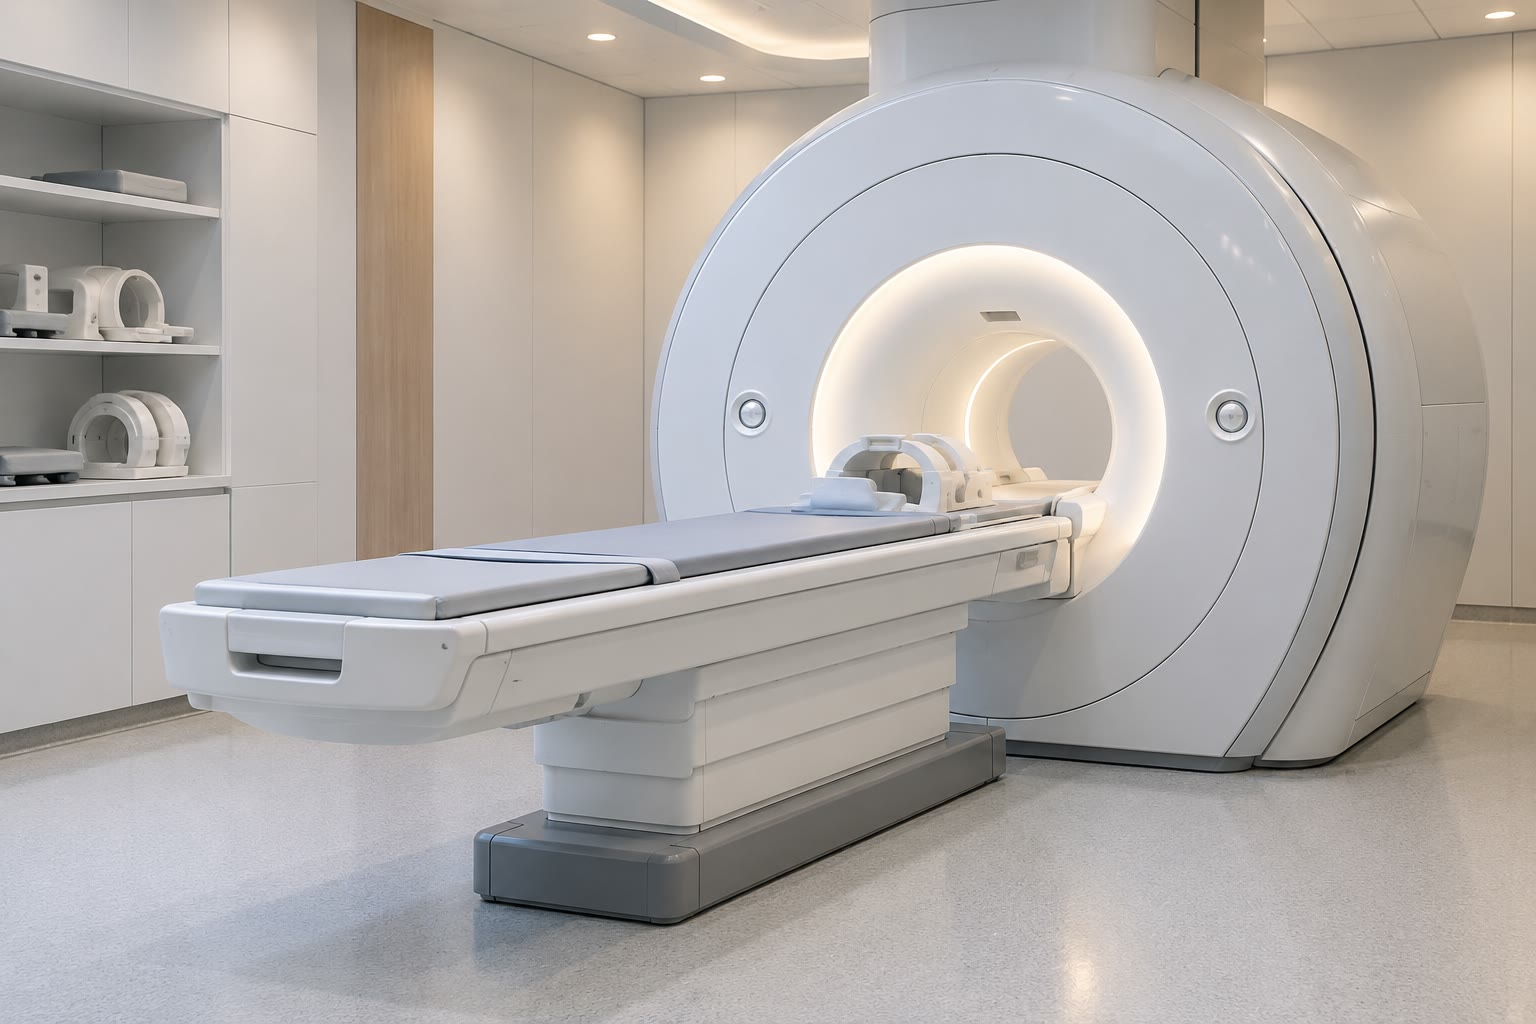
\includegraphics[width=0.52\linewidth]{images/book4/ai/b3-08-mri.jpg}\hspace{0.8em}%
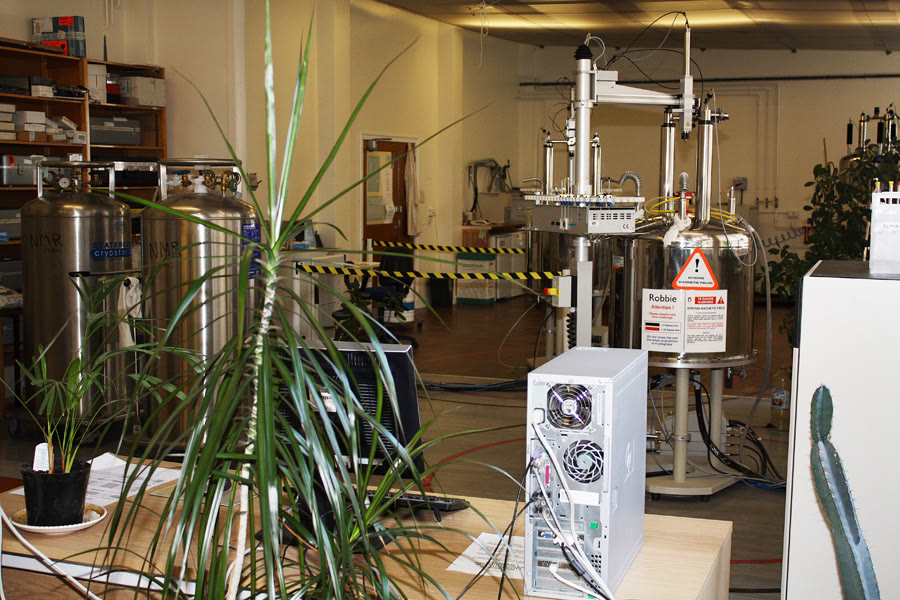
\includegraphics[width=0.4\linewidth]{images/book4/nmr-lab.jpg}

{\small बाएँ: अस्पताल का एक MRI स्कैनर। दाएँ: एक NMR प्रयोगशाला; हर
अतिचालक चुंबक अपने क्रायोस्टैट में खड़ा है, जिसे बाईं ओर के ड्युआर पात्रों से द्रव हीलियम
और द्रव नाइट्रोजन द्वारा पुनः भरा जाता है। (छायाचित्र: शैंडकेम,
CC BY 2.0।)}
\end{omfigure}

\section{चुंबकीय क्षेत्र में नाभिकीय चक्रण}

\begin{definition}[नाभिकीय चक्रण क्वांटम संख्या, घूर्णचुंबकीय अनुपात]\label{def:b3:advanced-nmr:nuclear-spin}
किसी नाभिक का चक्रण कोणीय संवेग होता है, जिसकी क्वांटम संख्या $I$ उसकी
\emph{नाभिकीय चक्रण क्वांटम संख्या}\index{नाभिकीय चक्रण क्वांटम संख्या} है ($I = 0$,
\ce{^{12}C}, \ce{^{16}O} के लिए; $\frac12$, \ce{^1H}, \ce{^{13}C}, \ce{^{15}N}, \ce{^{19}F},
\ce{^{31}P} के लिए; 1, \ce{^2H}, \ce{^{14}N} के लिए), और उसके समानुपाती एक चुंबकीय आघूर्ण $\boldsymbol\mu = \gamma\hat{\mathbf
I}$ होता है; $\gamma$ \emph{घूर्णचुंबकीय अनुपात}\index{घूर्णचुंबकीय अनुपात} है।
क्षेत्र $B_0$ (अक्ष $z$) के अनुदिश $\hat I_z$ मान $m_I\hbar$ लेता है,
$m_I = -I, \dots, I$।
\end{definition}

\begin{proposition}[ज़ेमान स्तर]\label{prop:b3:advanced-nmr:zeeman}
क्षेत्र $B_0$ में स्तर $E_m = -m_I\gamma\hbar B_0$ हैं; संक्रमण $\Delta m_I = \pm1$
इस आवृत्ति पर अवशोषण करते हैं:
\[
\nu_0 = \frac{\gamma B_0}{2\pi}.
\]
\end{proposition}

\begin{proof}
$E = -\boldsymbol\mu\cdot\mathbf B = -\gamma B_0\hat I_z$, जिसके \omterm{def:b3:quantum-model-systems:operator}{अभिलक्षणिक मान} $-\gamma B_0m_I\hbar$ हैं। सन्निकट
स्तरों का अंतर $\gamma\hbar B_0 = h\nu_0$ है।
\end{proof}

\begin{definition}[लार्मर आवृत्ति]\label{def:b3:advanced-nmr:larmor}
$\nu_0 = \gamma B_0/2\pi$ नाभिक की \emph{लार्मर आवृत्ति}\index{लार्मर आवृत्ति} है:
अनुनाद की आवृत्ति, और वह आवृत्ति भी जिस पर उसका
चुंबकीय आघूर्ण क्षेत्र के परितः पुरस्सरण करता है।
\end{definition}

\begin{example}[सामान्य नाभिक]\label{ex:b3:advanced-nmr:nuclei}
% ledger: const:gammaP, nuc:C13.mu, nuc:F19.mu, nuc:P31.mu, nuc:N15.mu, const:muN
चक्रण-$\frac12$ नाभिक के लिए, जिसका आघूर्ण $\mu$ है, $\gamma/2\pi = \mu/(Ih) = 2\mu/h$।
मापे गए आघूर्णों से: \ce{^1H} \qty{42.58}{MHz/T}, \ce{^{19}F} \qty{40.08}{MHz/T}, \ce{^{31}P}
\qty{17.25}{MHz/T}, \ce{^{13}C} \qty{10.71}{MHz/T}, \ce{^{15}N} \qty{-4.32}{MHz/T}। एक
``\qty{400}{MHz} स्पेक्ट्रममापी'' में $B_0 = \qty{9.4}{T}$ होता है: उसके प्रोटॉन
\qty{400.2}{MHz} पर अनुनाद करते हैं, उसके कार्बन \qty{100.7}{MHz} पर।
\end{example}

\begin{proposition}[समष्टि का अति सूक्ष्म अंतर]\label{prop:b3:advanced-nmr:populations}
चक्रण $\frac12$ के लिए, ताप $T$ पर, निचले स्तर में नाभिकों का आधिक्य यह है:
\[
\frac{N_\alpha - N_\beta}{N} \approx \frac{\gamma\hbar B_0}{2kT}.
\]
\end{proposition}

\begin{proof}
$N_\beta/N_\alpha = \eu^{-\Delta E/kT} \approx 1 - \Delta E/kT$, क्योंकि $\Delta E \ll kT$; अतः
$(N_\alpha - N_\beta)/(N_\alpha + N_\beta) \approx \Delta E/2kT$, जहाँ $\Delta E = \gamma\hbar B_0$।
\end{proof}

\qty{9.4}{T} और \qty{300}{K} पर प्रोटॉनों के लिए आधिक्य \num{3.2e-5} है: केवल
एक लाख में तीन नाभिक योगदान देते हैं। चूँकि आधिक्य और
कुंडली में प्रेरित वोल्टता दोनों $\gamma$ और $B_0$ के साथ बढ़ते हैं, संकेत
लगभग $\gamma^3B_0^2$ के रूप में बढ़ता है: यही कारण है सदा अधिक प्रबल चुंबकों का, और
छोटे $\gamma$ तथा कम प्राकृतिक प्रचुरता वाले नाभिकों, जैसे
\ce{^{13}C}, की कम संवेदनशीलता का।

\section{स्पंद और मुक्त प्रेरण क्षय}

\begin{definition}[नेट चुंबकन, घूर्णी निर्देश-तंत्र]\label{def:b3:advanced-nmr:magnetisation}
किसी नमूने का \emph{नेट चुंबकन}\index{नेट चुंबकन} $\mathbf M$, प्रति एकक आयतन
उसके नाभिकीय चुंबकीय आघूर्णों का योग है; साम्य पर वह
$M_0$ होता है, $\mathbf B_0$ के अनुदिश। \emph{घूर्णी निर्देश-तंत्र}\index{घूर्णी निर्देश-तंत्र}
अक्षों $x'$, $y'$, $z$ का ऐसा समुच्चय है जो प्रयुक्त रेडियो तरंगों की आवृत्ति पर $z$ के
परितः घूमता है; उसमें $\nu_0$ पर पुरस्सरण धीमा होकर अंतर $\nu_0 -
\nu_{\mathrm{rf}}$ के रूप में दिखता है।
\end{definition}

\begin{proposition}[पुरस्सरण]\label{prop:b3:advanced-nmr:precession}
क्षेत्र में चुंबकन $\dd\mathbf M/\dd t = \gamma\,\mathbf M\times\mathbf B$ का पालन करता है;
स्थैतिक क्षेत्र $B_0\mathbf e_z$ में उसका अनुप्रस्थ घटक $z$ के परितः कोणीय
आवृत्ति $\omega_0 = \gamma B_0$ पर घूमता है जबकि $M_z$ अचर रहता है।
\end{proposition}

\begin{proof}[आंशिक उपपत्ति]
यह समीकरण कोणीय संवेग वहन करने वाले चुंबकीय आघूर्ण के लिए चिरसम्मत बल-आघूर्ण
समीकरण है, जिसे भौतिकी से स्वीकार किया गया है। $\mathbf B = B_0\mathbf e_z$ के साथ: $\dot M_x = \gamma
B_0M_y$, $\dot M_y = -\gamma B_0M_x$, $\dot M_z = 0$, जिसका हल $M_x + \iu M_y \propto
\eu^{-\iu\gamma B_0t}$ है: $\omega_0$ पर एक घूर्णन ($+z$ से देखने पर दक्षिणावर्त, $\gamma > 0$ के लिए)।
\end{proof}

\begin{definition}[रेडियो-आवृत्ति स्पंद, पलट कोण]\label{def:b3:advanced-nmr:pulse}
\emph{रेडियो-आवृत्ति स्पंद}\index{रेडियो-आवृत्ति स्पंद}
$\nu_{\mathrm{rf}} \approx \nu_0$ पर रेडियो तरंगों का एक छोटा प्रस्फोट है, जिसका चुंबकीय क्षेत्र $B_1$,
\omterm{def:b3:advanced-nmr:magnetisation}{घूर्णी निर्देश-तंत्र} में $x'$ के अनुदिश स्थिर, $\mathbf M$ को $x'$ के परितः घुमाता है। घुमाया गया कोण
\emph{पलट कोण}\index{पलट कोण} $\theta = \gamma B_1t_p$ है, अवधि
$t_p$ वाले स्पंद के लिए: $90^\circ$ स्पंद $\mathbf M$ को $x'y'$ तल में लाता है, $180^\circ$ स्पंद
उसे उलट देता है।
\end{definition}

\begin{omfigure}
\tdplotsetmaincoords{70}{120}
\begin{tikzpicture}[tdplot_main_coords, font=\small, >=Stealth]
  \begin{scope}
    \draw[->, gray] (0,0,0) -- (1.8,0,0) node[anchor=north east] {$x'$};
    \draw[->, gray] (0,0,0) -- (0,1.8,0) node[anchor=north west] {$y'$};
    \draw[->, gray] (0,0,0) -- (0,0,1.8) node[anchor=south] {$z$, $\mathbf B_0$};
    \draw[->, omThm, very thick] (0,0,0) -- (0,0,1.4) node[anchor=west] {$\mathbf M$};
    \node[anchor=north] at (0,0,-0.9) {साम्य};
  \end{scope}
  \begin{scope}[shift={(0,4.6,0)}]
    \draw[->, gray] (0,0,0) -- (1.8,0,0) node[anchor=north east] {$x'$};
    \draw[->, gray] (0,0,0) -- (0,1.8,0) node[anchor=north west] {$y'$};
    \draw[->, gray] (0,0,0) -- (0,0,1.8) node[anchor=south] {$z$};
    \draw[->, omDef, thick] (0,0,0) -- (1.2,0,0) node[anchor=south east, xshift=-2pt] {$\mathbf B_1$};
    \draw[->, omThm, very thick] (0,0,0) -- (0,1.4,0) node[anchor=south west] {$\mathbf M$};
    \node[anchor=north] at (0,0,-0.9) {$90^\circ_{x'}$ स्पंद के बाद};
  \end{scope}
  \begin{scope}[shift={(0,9.2,0)}]
    \draw[->, gray] (0,0,0) -- (1.8,0,0) node[anchor=north east] {$x'$};
    \draw[->, gray] (0,0,0) -- (0,1.8,0) node[anchor=north west] {$y'$};
    \draw[->, gray] (0,0,0) -- (0,0,1.8) node[anchor=south] {$z$};
    \draw[->, omThm, very thick] (0,0,0) -- (0,0,-1.4) node[anchor=west] {$\mathbf M$};
    \node[anchor=north] at (0,0,-1.6) {$180^\circ_{x'}$ स्पंद के बाद};
  \end{scope}
\end{tikzpicture}

{\small \omterm{def:b3:advanced-nmr:magnetisation}{घूर्णी निर्देश-तंत्र} में चुंबकन। $90^\circ$ स्पंद, $x'$ के परितः,
$\mathbf M$ को $z$ से $y'$ पर घुमाता है ($\gamma > 0$ के साथ घूर्णन $\mathbf B_1$ के परितः
बाएँ हाथ के नियम का पालन करता है, जो सामान्य परिपाटी है); $180^\circ$ स्पंद
उसे उलट देता है।}
\end{omfigure}

\begin{definition}[मुक्त प्रेरण क्षय]\label{def:b3:advanced-nmr:fid}
$90^\circ$ स्पंद के बाद अनुप्रस्थ चुंबकन \omterm{def:b3:advanced-nmr:larmor}{लार्मर आवृत्ति} पर पुरस्सरण करता है
और नमूने के चारों ओर की कुंडली में एक दोलायमान वोल्टता प्रेरित करता है,
जो चुंबकन की विश्रांति के साथ मिटती जाती है: यही \emph{मुक्त प्रेरण
क्षय}\index{मुक्त प्रेरण क्षय} (FID) है।
\end{definition}

\begin{theorem}[FID से स्पेक्ट्रम तक]\label{thm:b3:advanced-nmr:lorentzian}
क्षीण होते दोलन $\eu^{-t/T_2}\cos(2\pi\nu t)$ ($t \ge 0$) का फ़ूरिये रूपांतर,
$\nu$ के निकट, अर्ध-अधिकतम पर पूर्ण चौड़ाई $1/(\pi T_2)$ वाली एक लॉरेंट्ज़ी रेखा है।
\end{theorem}

\begin{proof}
संकेत को $\eu^{-t/T_2}\eu^{2\pi\iu\nu t}$ लिखिए और समाकलन कीजिए:
$\int_0^\infty\eu^{-t/T_2}\eu^{2\pi\iu(\nu - f)t}\dd t = \frac{1}{1/T_2 - 2\pi\iu(\nu - f)}$, जिसका वास्तविक
भाग $\frac{T_2}{1 + 4\pi^2T_2^2(f - \nu)^2}$ है। यह $f = \nu$ पर अधिकतम है और
आधा तब होता है जब $2\pi T_2|f - \nu| = 1$, अर्थात् $f - \nu = \pm1/(2\pi T_2)$ पर: पूर्ण चौड़ाई
$1/(\pi T_2)$।
\end{proof}

\begin{omfigure}
\begin{tikzpicture}
\begin{axis}[name=fid, width=0.5\linewidth, height=4.6cm, xmin=0, xmax=0.4,
  ymin=-2.1, ymax=2.1, axis lines=left, xlabel={$t$ / s}, ylabel={संकेत},
  ytick=\empty, scaled x ticks=false, xticklabel style={/pgf/number format/fixed},
  tick label style={font=\small}, label style={font=\small}, title={\small FID}]
\addplot[omDef] table[x=t, y=s] {figdata/out/bachelor-3-nmr-fid.dat};
\addplot[gray, dashed, domain=0:0.4, samples=60] {2*exp(-x/0.1)};
\end{axis}
\begin{axis}[at={(fid.east)}, anchor=west, xshift=1.2cm, width=0.45\linewidth,
  height=4.6cm, xmin=0, xmax=350, ymin=-0.1, ymax=1.1, axis x line=bottom,
  axis y line=none, xlabel={अंतर / Hz}, tick label style={font=\small},
  label style={font=\small}, title={\small स्पेक्ट्रम (फ़ूरिये रूपांतर)}]
\addplot[omThm, thick] table[x=f, y=I] {figdata/out/bachelor-3-nmr-fid-spectrum.dat};
\end{axis}
\end{tikzpicture}

{\small बाएँ: दो रेखाओं का FID (अंतर 100 और \qty{250}{Hz}, $T_2 = \qty{0.10}{s}$),
जो एक चरघातांकी आवरण (खंडित) के भीतर दोनों आवृत्तियों के व्यतिकरण से विस्पंदित होता है।
दाएँ: उसका फ़ूरिये रूपांतर, \qty{3.2}{Hz} चौड़ी दो लॉरेंट्ज़ी रेखाएँ।}
\end{omfigure}

\begin{proposition}[संकेत औसतन]\label{prop:b3:advanced-nmr:averaging}
$N$ FID जोड़ने से संकेत $N$ गुना और यादृच्छिक रव $\sqrt N$ गुना हो जाता है:
संकेत-रव अनुपात $\sqrt N$ के रूप में बढ़ता है।
\end{proposition}

\begin{proof}
संकेत संबद्ध रूप से जुड़ता है। स्वतंत्र अधिग्रहणों के रव का माध्य शून्य
और हर एक का प्रसरण $\sigma^2$ है; $N$ स्वतंत्र पदों के योग का प्रसरण
$N\sigma^2$ है (द्वितीय वर्ष के खंड का संचरण नियम), अतः उसका मानक विचलन
$\sqrt N\sigma$ है।
\end{proof}

DEPT, जो ${}^{13}$C संकेतों को संलग्न हाइड्रोजनों की संख्या के अनुसार छाँटता है,
प्रोटॉनों और कार्बनों दोनों पर स्पंदों का एक अनुक्रम लगाता है, जो
$1/2J$ के विलंबों से अलग होते हैं: प्रोटॉन का बड़ा चुंबकन एक-आबंध युग्मन के माध्यम से
कार्बन में स्थानांतरित होता है, जिससे कार्बन संकेत लगभग
$\gamma_H/\gamma_C \approx 4$ गुना हो जाता है, और अंतिम प्रोटॉन स्पंद का कोण CH, \ce{CH2} और
\ce{CH3} को भिन्न भार देता है। यही विचार --- नाभिकों के बीच उनके युग्मनों के माध्यम से
चुंबकन का स्थानांतरण --- आगे के द्विविमीय प्रयोगों का आधार है।

\section{विश्रांति}

\begin{definition}[अनुदैर्घ्य और अनुप्रस्थ विश्रांति काल]\label{def:b3:advanced-nmr:relaxation}
किसी विक्षोभ के बाद $M_z$ का $M_0$ पर लौटना चरघातांकी है,
\emph{अनुदैर्घ्य विश्रांति काल}\index{अनुदैर्घ्य विश्रांति काल} $T_1$ के साथ
(चक्रण--जालक विश्रांति: परिवेश को दी गई ऊर्जा)। अनुप्रस्थ चुंबकन का
शून्य तक क्षय चरघातांकी है,
\emph{अनुप्रस्थ विश्रांति काल}\index{अनुप्रस्थ विश्रांति काल} $T_2 \le T_1$ के साथ
(चक्रण--चक्रण विश्रांति: चक्रणों के बीच कला-संबद्धता की हानि)।
\end{definition}

\begin{proposition}[प्रतिलोमन पुनःप्राप्ति]\label{prop:b3:advanced-nmr:inversion-recovery}
$180^\circ$ स्पंद के बाद $M_z(t) = M_0(1 - 2\eu^{-t/T_1})$; यह
$t_{\mathrm{null}} = T_1\ln2$ पर शून्य से होकर गुज़रता है।
\end{proposition}

\begin{proof}
विश्रांति समीकरण $\dd M_z/\dd t = (M_0 - M_z)/T_1$, जहाँ $M_z(0) = -M_0$, का
हल $M_0 - 2M_0\eu^{-t/T_1}$ है, जो तब लुप्त होता है जब $\eu^{-t/T_1} = \frac12$।
\end{proof}

\begin{method}[$T_1$ मापना और मात्रात्मक पुनरावर्तन विलंब निर्धारित करना]\label{met:b3:advanced-nmr:t1}
\begin{enumerate}
  \item अनुक्रम $180^\circ$--$\tau$--$90^\circ$--अधिग्रहण को विलंबों $\tau$ की एक श्रेणी के लिए
        चलाइए, स्कैनों के बीच कम से कम $5T_1$ प्रतीक्षा करते हुए।
  \item हर संकेत को $M_0(1 - 2\eu^{-\tau/T_1})$ पर समंजित कीजिए, या शून्य-बिंदु पढ़िए: $T_1 =
        t_{\mathrm{null}}/\ln2$।
  \item $90^\circ$ स्पंदों के साथ मात्रात्मक समाकलन के लिए स्कैनों के बीच सबसे धीमे नाभिक के
        $5T_1$ की कम से कम प्रतीक्षा कीजिए: तब चुंबकन का $\eu^{-5} < 1\,\%$ भाग ही
        छूटता है।
\end{enumerate}
\end{method}

\begin{omfigure}
\begin{tikzpicture}
\begin{axis}[width=0.62\linewidth, height=5cm, xmin=0, xmax=10, ymin=-1.1, ymax=1.15,
  axis lines=left, xlabel={$t$ / s}, ylabel={$M/M_0$}, legend cell align=left,
  legend style={font=\small, draw=none, at={(0.97,0.05)}, anchor=south east},
  tick label style={font=\small}, label style={font=\small}]
\addplot[omDef, thick] table[x=t, y=mz] {figdata/out/bachelor-3-nmr-relaxation.dat};
\addlegendentry{$M_z$, $180^\circ$ के बाद ($T_1 = \qty{2.0}{s}$)}
\addplot[omThm, thick, dashed] table[x=t, y=mxy] {figdata/out/bachelor-3-nmr-relaxation.dat};
\addlegendentry{$M_{xy}$, $90^\circ$ के बाद ($T_2 = \qty{0.5}{s}$)}
\addplot[gray, dotted, domain=0:10] {0};
\addplot[only marks, mark=*, mark size=1.5pt, black] coordinates {(1.386,0)};
\node[font=\small, anchor=north west] at (axis cs:1.5,-0.04) {$T_1\ln2$};
\end{axis}
\end{tikzpicture}

{\small विश्रांति (मॉडल मान)। प्रतिलोमित अनुदैर्घ्य चुंबकन
$T_1\ln2$ पर शून्य से होकर पुनः प्राप्त होता है; अनुप्रस्थ चुंबकन
तेज़ी से, $T_2$ के साथ, क्षीण होता है।}
\end{omfigure}

\begin{definition}[चक्रण प्रतिध्वनि]\label{def:b3:advanced-nmr:echo}
अनुक्रम $90^\circ$--$\tau$--$180^\circ$--$\tau$ में, जो चक्रण क्षेत्र की असमांगताओं के कारण कला में
अलग हो गए थे, वे समय $2\tau$ पर पुनः केंद्रित हो जाते हैं, और एक
\emph{चक्रण प्रतिध्वनि}\index{चक्रण प्रतिध्वनि} उत्पन्न करते हैं; उसका आयाम वास्तविक $T_2$ के साथ
क्षीण होता है, चुंबक की असमांगता से मुक्त।
\end{definition}

\begin{definition}[नाभिकीय ओवरहाउज़र प्रभाव]\label{def:b3:advanced-nmr:noe}
किसी एक चक्रण को संतृप्त या विक्षुब्ध करने से, उनकी द्विध्रुवी
विश्रांति के माध्यम से, आकाश में निकट स्थित किसी अन्य चक्रण के संकेत की तीव्रता बदल जाती है:
यही \emph{नाभिकीय ओवरहाउज़र प्रभाव}\index{नाभिकीय ओवरहाउज़र प्रभाव} (NOE) है।
उसके विकास की दर $r^{-6}$ के समानुपाती है, अतः वह केवल लगभग \qty{0.5}{nm} से कम दूरी
वाले नाभिकों के बीच दिखता है, चाहे वे आबंधित हों या नहीं।
\end{definition}

\section{द्विविमीय NMR}

\begin{definition}[द्विविमीय स्पेक्ट्रम, तिर्यक शिखर, विकर्ण शिखर]\label{def:b3:advanced-nmr:two-d}
\emph{द्विविमीय स्पेक्ट्रम}\index{द्विविमीय स्पेक्ट्रम} एक स्पंद अनुक्रम को,
एक बढ़ाए गए विलंब $t_1$ के साथ, जो अधिग्रहण काल $t_2$ से पहले आता है, दोहराकर
अभिलिखित किया जाता है; दोहरा फ़ूरिये रूपांतर दो आवृत्तियों के विरुद्ध
तीव्रता का एक मानचित्र देता है। $(\delta_1,
\delta_2)$ पर \emph{तिर्यक शिखर}\index{तिर्यक शिखर} दिखाता है कि $\delta_1$ और $\delta_2$ पर स्थित नाभिक
(किसी युग्मन या निकटता से) जुड़े हैं; $(\delta, \delta)$ पर \emph{विकर्ण शिखर}\index{विकर्ण शिखर}
एक ही नाभिक का होता है।
\end{definition}

\begin{definition}[COSY, HSQC, HMBC, NOESY]\label{def:b3:advanced-nmr:experiments}
\emph{COSY}\index{COSY} (सहसंबंध स्पेक्ट्रमिकी) एक-दूसरे से युग्मित प्रोटॉनों को
सहसंबद्ध करता है, प्रायः तीन आबंधों के पार (H--C--C--H)। \emph{HSQC}\index{HSQC}
(विषमनाभिकीय एकल-क्वांटम संबद्धता) हर कार्बन को उससे प्रत्यक्ष आबंधित
प्रोटॉनों से सहसंबद्ध करता है। \emph{HMBC}\index{HMBC} (विषमनाभिकीय
बहु-आबंध सहसंबंध) कार्बनों को दो या तीन आबंध दूर स्थित प्रोटॉनों से सहसंबद्ध करता है,
चतुष्क कार्बनों और विषमपरमाणुओं के पार भी। \emph{NOESY}\index{NOESY}
आकाश में निकट स्थित प्रोटॉनों को \omterm{def:b3:advanced-nmr:noe}{नाभिकीय ओवरहाउज़र प्रभाव} के माध्यम से सहसंबद्ध करता है।
\end{definition}

\begin{omfigure}
\begin{tikzpicture}[font=\small]
  \foreach \y/\name in {3.2/{एक स्पंद}, 2.0/{प्रतिलोमन पुनःप्राप्ति}, 0.8/{चक्रण प्रतिध्वनि}, -0.4/{COSY}}{
    \draw (0,\y) -- (9.3,\y); \node[anchor=east] at (-0.1,\y+0.25) {\name};}
  % one pulse
  \fill[black] (0.4,3.2) rectangle (0.6,3.75);
  \draw[omDef, domain=0:3.5, samples=120] plot (0.7+\x, {3.2+0.4*exp(-\x/1.2)*sin(\x*500)});
  % inversion recovery
  \fill[black] (0.4,2.0) rectangle (0.8,2.55); \node[font=\scriptsize] at (0.6,2.7) {180};
  \draw[<->] (0.85,1.85) -- (2.4,1.85) node[midway, below, font=\scriptsize] {$\tau$};
  \fill[black] (2.45,2.0) rectangle (2.65,2.55); \node[font=\scriptsize] at (2.55,2.7) {90};
  \draw[omDef, domain=0:3.0, samples=120] plot (2.75+\x, {2.0+0.4*exp(-\x/1.0)*sin(\x*500)});
  % spin echo
  \fill[black] (0.4,0.8) rectangle (0.6,1.35); \node[font=\scriptsize] at (0.5,1.5) {90};
  \draw[<->] (0.65,0.65) -- (2.4,0.65) node[midway, below, font=\scriptsize] {$\tau$};
  \fill[black] (2.45,0.8) rectangle (2.85,1.35); \node[font=\scriptsize] at (2.65,1.5) {180};
  \draw[<->] (2.9,0.65) -- (4.65,0.65) node[midway, below, font=\scriptsize] {$\tau$};
  \draw[omDef, domain=-1.2:2.5, samples=150] plot (4.65+\x, {0.8+0.35*exp(-abs(\x)/0.35)*cos(\x*700)});
  % COSY
  \fill[black] (0.4,-0.4) rectangle (0.6,0.15); \node[font=\scriptsize] at (0.5,0.3) {90};
  \draw[<->] (0.65,-0.55) -- (2.4,-0.55) node[midway, below, font=\scriptsize] {$t_1$ (बढ़ाया गया)};
  \fill[black] (2.45,-0.4) rectangle (2.65,0.15); \node[font=\scriptsize] at (2.55,0.3) {90};
  \draw[omDef, domain=0:3.0, samples=120] plot (2.75+\x, {-0.4+0.4*exp(-\x/1.0)*sin(\x*500)});
  \node[font=\scriptsize, anchor=west] at (5.9,-0.2) {अधिग्रहण ($t_2$)};
\end{tikzpicture}

{\small स्पंद अनुक्रम (समय दाईं ओर; भरे हुए खाने: स्पंद, जिन पर
उनके \omterm{def:b3:advanced-nmr:pulse}{पलट कोण} अंशों में अंकित हैं; नीला: अभिलिखित संकेत)। \omterm{def:b3:advanced-nmr:echo}{चक्रण प्रतिध्वनि}
पहले स्पंद के $2\tau$ बाद शिखर पर होती है।}
\end{omfigure}

\begin{method}[द्विविमीय स्पेक्ट्रमों से संरचना हल करना]\label{met:b3:advanced-nmr:solve-2d}
\begin{enumerate}
  \item सूत्र, ${}^1$H समाकलों और ${}^{13}$C/DEPT स्पेक्ट्रम से
        CH, \ce{CH2}, \ce{CH3} और चतुष्क कार्बनों को सूचीबद्ध कीजिए।
  \item \omterm{def:b3:advanced-nmr:experiments}{HSQC}: हर प्रोटॉन संकेत को उसके कार्बन से जोड़िए।
  \item \omterm{def:b3:advanced-nmr:experiments}{COSY}: प्रोटॉनित कार्बनों को चक्रण तंत्रों (पड़ोसियों की
        शृंखलाओं) में जोड़िए।
  \item \omterm{def:b3:advanced-nmr:experiments}{HMBC}: चक्रण तंत्रों को चतुष्क कार्बनों, कार्बोनिलों और
        विषमपरमाणुओं के पार जोड़िए, जहाँ \omterm{def:b3:advanced-nmr:experiments}{COSY} मूक है।
  \item \omterm{def:b3:advanced-nmr:experiments}{NOESY}: आकाश के माध्यम से संपर्कों से आपेक्षिक विन्यास और संरूपण
        निर्धारित कीजिए।
  \item हर संकेत को प्रस्तावित संरचना के विरुद्ध जाँचिए।
\end{enumerate}
\end{method}

\begin{omfigure}
\begin{tikzpicture}
\begin{axis}[name=cosy, width=0.47\linewidth, height=0.47\linewidth, x dir=reverse,
  y dir=reverse, xmin=0.5, xmax=4.6, ymin=0.5, ymax=4.6, axis lines=box,
  xlabel={$\delta_{\mathrm H}$ / ppm}, ylabel={$\delta_{\mathrm H}$ / ppm},
  tick label style={font=\small}, label style={font=\small}, title={\small COSY}]
\addplot[gray, dotted, domain=0.5:4.6] {x};
\addplot[only marks, mark=*, mark size=2.2pt, black] table[x=h1, y=h2] {figdata/out/bachelor-3-nmr-2d-cosy-diag.dat};
\addplot[only marks, mark=*, mark size=2.2pt, omThm] table[x=h1, y=h2] {figdata/out/bachelor-3-nmr-2d-cosy-cross.dat};
\end{axis}
\begin{axis}[at={(cosy.east)}, anchor=west, xshift=1.3cm, width=0.47\linewidth,
  height=0.47\linewidth, x dir=reverse, y dir=reverse, xmin=0.5, xmax=4.6,
  ymin=0, ymax=185, axis lines=box, xlabel={$\delta_{\mathrm H}$ / ppm},
  ylabel={$\delta_{\mathrm C}$ / ppm}, tick label style={font=\small},
  label style={font=\small}, title={\small HSQC (नीला) और HMBC (लाल)}]
\addplot[only marks, mark=square*, mark size=2.2pt, omDef] table[x=h, y=c] {figdata/out/bachelor-3-nmr-2d-hsqc.dat};
\addplot[only marks, mark=o, mark size=2.6pt, omThm, thick] table[x=h, y=c] {figdata/out/bachelor-3-nmr-2d-hmbc.dat};
\end{axis}
\end{tikzpicture}

{\small एथिल ब्यूटेनोएट, \ce{CH3CH2CH2COOCH2CH3}, के \omterm{def:b3:advanced-nmr:two-d}{द्विविमीय स्पेक्ट्रम},
उसके मापे गए विस्थापनों पर खींचे गए। \omterm{def:b3:advanced-nmr:experiments}{COSY}: काले, \omterm{def:b3:advanced-nmr:two-d}{विकर्ण शिखर}; लाल, पड़ोसी कार्बनों
पर स्थित प्रोटॉनों के बीच \omterm{def:b3:advanced-nmr:two-d}{तिर्यक शिखर} --- दो चक्रण तंत्र, एथिल और
प्रोपिल, एस्टर ऑक्सीजन के पार कोई \omterm{def:b3:advanced-nmr:two-d}{तिर्यक शिखर} नहीं। दाएँ: \omterm{def:b3:advanced-nmr:experiments}{HSQC} शिखर
(वर्ग) हर प्रोटॉन को उसके कार्बन से जोड़ते हैं; \omterm{def:b3:advanced-nmr:experiments}{HMBC} शिखर (वृत्त) दिखाते हैं कि OCH$_2$
प्रोटॉन (\qty{4.13}{ppm}) और CH$_2$C=O प्रोटॉन (\qty{2.28}{ppm}) दोनों
\qty{173.6}{ppm} पर स्थित कार्बोनिल कार्बन तक पहुँचते हैं।}
\end{omfigure}

\section{अन्य नाभिक और गतिकी}

फ़्लुओरीन-19 और फ़ॉस्फ़ोरस-31, जो चक्रण $\frac12$ वाले, 100\,\% प्रचुर और बड़े
$\gamma$ वाले हैं, लगभग प्रोटॉनों जितनी ही आसानी से प्रेक्षित होते हैं; उनके विस्थापनों की विस्तृत परासें
उन्हें अपने परिवेश (औषधियाँ, फ़ॉस्फ़ेट, \cref{ch:b3:organometallic-bonding} के फ़ॉस्फ़ीन जैसे
लिगैंड) के परिशुद्ध अन्वेषी बनाती हैं। नाइट्रोजन-15 दुर्लभ और
दुर्बल है, और प्रायः उससे आबंधित प्रोटॉनों के माध्यम से अप्रत्यक्ष रूप से प्रेक्षित किया जाता है।
भिन्न नाभिकों के बीच युग्मन वियुग्मन द्वारा हटाया जाता है, जैसा द्वितीय वर्ष के खंड में
${}^{13}$C के लिए।

\begin{definition}[संगलन ताप]\label{def:b3:advanced-nmr:coalescence}
जब कोई नाभिक दो ऐसे परिवेशों के बीच विनिमय करता है जिनके विस्थापनों का अंतर
$\Delta\nu$ (हर्ट्ज़ में) है, तो विनिमय तीव्र होने पर उसकी दोनों रेखाएँ चौड़ी होती हैं और
\emph{संगलन ताप}\index{संगलन ताप}
$T_c$ पर एक में मिल जाती हैं।
\end{definition}

\begin{proposition}[संगलन पर दर]\label{prop:b3:advanced-nmr:coalescence}
युग्मन रहित, समान रूप से समष्टित दो स्थलों के लिए संगलन पर विनिमय दर स्थिरांक
$k_c = \pi\Delta\nu/\sqrt2$ है।
\end{proposition}
\admitted

व्युत्पत्ति, विनिमय सहित ब्लॉख समीकरणों से, अधिक उन्नत पाठ्यक्रमों में
दी जाती है। आयरिंग समीकरण (\cref{ch:b3:rate-theories}) के साथ दर
अवरोध देती है: गतिक NMR ऐमाइड आबंधों के परितः घूर्णन, वलय-पलटन
और लिगैंड विनिमय मापता है, जिनके अवरोध 40 से \qty{100}{kJ/mol} तक होते हैं।

\begin{example}[एक MRI प्रतिबिंब]\label{ex:b3:advanced-nmr:mri}
चुंबकीय अनुनाद प्रतिबिंबन में एक क्षेत्र प्रवणता जल प्रोटॉनों की \omterm{def:b3:advanced-nmr:larmor}{लार्मर आवृत्ति} को
स्थिति पर निर्भर बना देती है, ताकि संकेत का फ़ूरिये रूपांतर इसका
मानचित्र हो कि वे कहाँ हैं। विषमता विश्रांति से आती है:
पुनरावृत्ति काल और प्रतिध्वनि विलंब इस प्रकार चुने जाते हैं कि प्रतिबिंब $T_1$ या
$T_2$ से भारित हो, जो ऊतकों के बीच भिन्न होते हैं; गैडोलिनियम युक्त विषमता कारक
निकटवर्ती जल का $T_1$ घटा देते हैं (\cref{ch:b3:bioinorganic})।
\end{example}

\begin{inthelab}[स्पेक्ट्रममापी को तैयार करना]
ड्यूटेरीकृत विलायक में घुला नमूना प्रोब में उतारा जाता है।
क्षेत्र के धीमे विचलन की क्षतिपूर्ति के लिए स्पेक्ट्रममापी ड्यूटेरियम संकेत पर लॉक होता है;
प्रोब को हर नाभिक की आवृत्ति के अनुसार समस्वरित और सुमेलित किया जाता है;
शिम कुंडलियों को तब तक समायोजित करके नमूने पर क्षेत्र को समांग बनाया जाता है
जब तक रेखाएँ संकीर्ण न हो जाएँ। चुंबक का क्षेत्र स्थायी है: इस्पात के औज़ार,
क्रेडिट कार्ड और पेसमेकर चिह्नित सुरक्षा रेखा के बाहर रखे जाते हैं।
\end{inthelab}

\begin{history}[अनुनाद से दो विमाओं तक]
फ़ेलिक्स ब्लॉख और एडवर्ड पर्सेल ने 1946 में स्थूल द्रव्य में नाभिकीय चुंबकीय अनुनाद
का संसूचन किया (भौतिकी का नोबेल पुरस्कार, 1952)। रिचर्ड अर्न्स्ट ने 1966 में स्पंदित
फ़ूरिये-रूपांतर NMR प्रारंभ किया और, ज़्याँ ज़ेनर के एक विचार का अनुसरण करते हुए,
1970 के दशक में द्विविमीय स्पेक्ट्रमिकी (रसायन का नोबेल पुरस्कार, 1991)।
\end{history}

\section{अभ्यास}

\begin{exercise}[$\star$]\label{exo:b3:advanced-nmr:1}
% ledger: const:gammaP, nuc:C13.mu, nuc:F19.mu
\qty{14.1}{T} पर \ce{^1H}, \ce{^{13}C} और \ce{^{19}F} की \omterm{def:b3:advanced-nmr:larmor}{लार्मर आवृत्तियाँ} परिकलित कीजिए
($\gamma/2\pi = 42.58$, 10.71 और \qty{40.08}{MHz/T})।
\end{exercise}

\begin{exercise}[$\star$]\label{exo:b3:advanced-nmr:2}
\qty{9.4}{T} और \qty{300}{K} पर निचले स्तर में प्रोटॉनों का आपेक्षिक आधिक्य परिकलित कीजिए।
\qty{4}{K} पर यह कितना बदल जाता है?
\end{exercise}

\begin{exercise}[$\star$]\label{exo:b3:advanced-nmr:3}
प्रोटॉनों के लिए $90^\circ$ स्पंद \qty{10}{\micro s} तक चलता है। $\gamma B_1/2\pi$ क्या है?
$180^\circ$ स्पंद कितना लंबा है, और \qty{5}{\micro s} का स्पंद क्या करता है?
\end{exercise}

\begin{exercise}[$\star$]\label{exo:b3:advanced-nmr:4}
एक रेखा अर्ध-ऊँचाई पर \qty{3.2}{Hz} चौड़ी है। $T_2$ क्या है (पूर्णतः
समांग क्षेत्र मानते हुए)?
\end{exercise}

\begin{exercise}[$\star\star$]\label{exo:b3:advanced-nmr:5}
% ledger: iso:C13
प्रति नाभिक संकेत $\propto\gamma^3$ और \ce{^{13}C} की 1.1\,\% प्राकृतिक प्रचुरता का
उपयोग करके ${}^{13}$C और ${}^1$H NMR की संवेदनशीलता की तुलना कीजिए। समान संकेत-रव अनुपात के लिए
${}^{13}$C स्पेक्ट्रम को कितने गुना अधिक स्कैन चाहिए?
\end{exercise}

\begin{exercise}[$\star\star$]\label{exo:b3:advanced-nmr:6}
एक प्रतिलोमन-पुनःप्राप्ति प्रयोग में किसी कार्बन का संकेत
$\tau = \qty{1.39}{s}$ पर लुप्त हो जाता है। $T_1$ और मात्रात्मक कार्य के लिए पुनरावर्तन विलंब ज्ञात कीजिए।
\end{exercise}

\begin{exercise}[$\star\star$]\label{exo:b3:advanced-nmr:7}
ब्यूटेनोन, \ce{CH3COCH2CH3}, के \omterm{def:b3:advanced-nmr:experiments}{COSY} स्पेक्ट्रम में कौन-से \omterm{def:b3:advanced-nmr:two-d}{तिर्यक शिखर} दिखते हैं?
एकक मेथिल प्रोटॉनों से कौन-से कार्बन \omterm{def:b3:advanced-nmr:experiments}{HMBC} शिखर दिखाते हैं?
\end{exercise}

\begin{exercise}[$\star\star$]\label{exo:b3:advanced-nmr:8}
किसी ऐमाइड के दो मेथिल संकेत, जो निम्न ताप पर \qty{50}{Hz} अलग हैं,
\qty{330}{K} पर संगलित होते हैं। संगलन पर विनिमय दर और सक्रियण की गिब्स ऊर्जा
परिकलित कीजिए, $\Delta G^\ddagger = RT_c\ln(k_BT_c/hk_c)$ के साथ।
\end{exercise}

\begin{exercise}[$\star\star$]\label{exo:b3:advanced-nmr:9}
प्रोटॉनों H$_a$ और H$_b$ के बीच NOE, H$_a$ और
H$_c$ के बीच वाले से चार गुना प्रबल है, जो \qty{0.30}{nm} पर हैं। H$_a$--H$_b$ दूरी का आकलन कीजिए।
\end{exercise}

\begin{exercise}[$\star\star\star$]\label{exo:b3:advanced-nmr:10}
\omterm{def:b3:advanced-nmr:magnetisation}{घूर्णी निर्देश-तंत्र} में $\dd\mathbf M/\dd t = \gamma\mathbf M\times\mathbf B_1$ को हल करके,
$\mathbf B_1$ को $x'$ के अनुदिश लेते हुए, दिखाइए कि स्पंद $\mathbf M$ को $\gamma B_1t_p$ से $x'$ के परितः घुमाता है।
\end{exercise}

\begin{exercise}[$\star\star\star$]\label{exo:b3:advanced-nmr:11}
समझाइए कि \omterm{def:b3:advanced-nmr:echo}{चक्रण प्रतिध्वनि} असमांग क्षेत्र के कारण हुए कला-विचलन को पुनः केंद्रित
क्यों करती है परंतु चक्रणों के बीच यादृच्छिक अन्योन्यक्रियाओं के कारण हुए विचलन को नहीं। प्रतिध्वनि का
आयाम कौन-सा काल-स्थिरांक मापता है?
\end{exercise}

\begin{exercise}[$\star\star\star$]\label{exo:b3:advanced-nmr:12}
\ce{C4H8O2} यौगिक की संरचना प्रस्तावित कीजिए जिसका ${}^1$H स्पेक्ट्रम एक
चतुष्क (2H, 4.12 ppm), एक एकक (3H, 2.05 ppm) और एक त्रिक (3H,
1.26 ppm) दिखाता है, और जिसका \omterm{def:b3:advanced-nmr:experiments}{HMBC} स्पेक्ट्रम चतुष्क प्रोटॉनों को
171 ppm पर स्थित एक कार्बन से सहसंबद्ध करता है (अभ्यास के आँकड़े)। उसी सूत्र का कौन-सा
दूसरा एस्टर भिन्न \omterm{def:b3:advanced-nmr:experiments}{HMBC} पैटर्न देगा, और कैसे?
\end{exercise}

\section{समस्या: दो विमाओं में अनन्नास का एस्टर}

\begin{problem}[{सप्ताहांत समस्या --- द्विविमीय स्पेक्ट्रमों से एथिल ब्यूटेनोएट फिर से हल करना:
COSY से चक्रण तंत्र, HSQC से कार्बन, HMBC से
एस्टर बंधन, और मात्रात्मक कार्बन स्पेक्ट्रम के लिए आवश्यक
विलंब}]
\label{pb:b3:advanced-nmr:1}
% ledger: nmr:ethylbutanoate-OCH2, nmr:ethylbutanoate-CH2CO, nmr:ethylbutanoate-CH2, nmr:ethylbutanoate-OCH2CH3, nmr:ethylbutanoate-CH3, c13:ethylbutanoate.CO, c13:ethylbutanoate.OCH2, c13:ethylbutanoate.CH2CO, c13:ethylbutanoate.CH2, c13:ethylbutanoate.OCH2CH3, c13:ethylbutanoate.CH3
अनन्नास की सुगंध से प्राप्त एक एस्टर \ce{C6H12O2} ${}^1$H संकेत 4.13 (2H,
चतुष्क), 2.28 (2H, त्रिक), 1.66 (2H, बहुक), 1.25 (3H, त्रिक) और 0.95 ppm (3H, त्रिक) पर, और ${}^{13}$C संकेत
173.6, 60.1, 36.3, 18.6, 14.3 और 13.7 ppm पर दिखाता है, जो \qty{9.4}{T} पर अभिलिखित हैं। उसके \omterm{def:b3:advanced-nmr:two-d}{द्विविमीय
स्पेक्ट्रम} अनुभाग 4 के चित्र वाले हैं। समस्या के आँकड़े: कार्बनों के $T_1$
मान कार्बोनिल के लिए लगभग \qty{20}{s} और बाकी के लिए 2 से \qty{6}{s} हैं।

\medskip\noindent\textbf{भाग I --- एक विमा।}
\begin{enumerate}
  \item \ce{C6H12O2} की असंतृप्ति की मात्रा परिकलित कीजिए।
  \item कौन-सा ${}^{13}$C संकेत कार्बोनिल है? कौन-सा ऑक्सीजन से आबंधित कार्बन है?
  \item कितने प्रोटॉनित कार्बन हैं? DEPT-135 क्या दिखाएगा?
  \item \qty{9.4}{T} पर ${}^1$H और ${}^{13}$C की \omterm{def:b3:advanced-nmr:larmor}{लार्मर आवृत्तियाँ} क्या हैं?
  \item चतुष्क का युग्मन \qty{7.2}{Hz} है। \qty{400}{MHz} पर चतुष्क ppm में कितना
        चौड़ा है?
  \item केवल एकविमीय स्पेक्ट्रम अणुखंडों का क्रम अनिर्धारित क्यों छोड़ सकते हैं?
\end{enumerate}

\medskip\noindent\textbf{भाग II --- \omterm{def:b3:advanced-nmr:experiments}{COSY}।}
\begin{enumerate}[resume]
  \item \omterm{def:b3:advanced-nmr:experiments}{COSY} मानचित्र के \omterm{def:b3:advanced-nmr:two-d}{तिर्यक शिखर} सूचीबद्ध कीजिए।
  \item दोनों चक्रण तंत्र निकालिए।
  \item 4.13 और 2.28 ppm के बीच कोई \omterm{def:b3:advanced-nmr:two-d}{तिर्यक शिखर} क्यों नहीं है?
  \item कौन-सा प्रोटॉन संकेत दो अन्य से युग्मित है? उसकी बहुकता समझाइए।
  \item 0.95 और 1.25 ppm के बीच \omterm{def:b3:advanced-nmr:two-d}{तिर्यक शिखर} का क्या अर्थ होता?
  \item दोनों अणुखंड खींचिए।
\end{enumerate}

\medskip\noindent\textbf{भाग III --- \omterm{def:b3:advanced-nmr:experiments}{HSQC} और \omterm{def:b3:advanced-nmr:experiments}{HMBC}।}
\begin{enumerate}[resume]
  \item \omterm{def:b3:advanced-nmr:experiments}{HSQC} से हर कार्बन को उसके प्रोटॉनों से निर्दिष्ट कीजिए।
  \item कौन-से दो मेथिल कार्बन केवल \omterm{def:b3:advanced-nmr:experiments}{HSQC} से विभेदित होते हैं?
  \item कौन-सा \omterm{def:b3:advanced-nmr:experiments}{HMBC} शिखर एथिल अणुखंड को कार्बोनिल से जोड़ता है, और
        कितने आबंधों के पार?
  \item कौन-से \omterm{def:b3:advanced-nmr:experiments}{HMBC} शिखर प्रोपिल अणुखंड को कार्बोनिल से जोड़ते हैं?
  \item संरचना निकालिए, और उसके समावयवी प्रोपिल प्रोपेनोएट को अस्वीकार कीजिए।
  \item चार या अधिक आबंधों के पार \omterm{def:b3:advanced-nmr:experiments}{HMBC} शिखर प्रायः अनुपस्थित क्यों होते हैं?
\end{enumerate}

\medskip\noindent\textbf{भाग IV --- एक मात्रात्मक कार्बन स्पेक्ट्रम।}
\begin{enumerate}[resume]
  \item सामान्य ${}^{13}$C स्पेक्ट्रम के समाकल कार्बनों की संख्या के समानुपाती
        क्यों नहीं होते?
  \item यदि $90^\circ$ स्पंदों के साथ हर \qty{5}{s} पर स्कैन दोहराए जाएँ (हर बार
        शून्य से आरंभ करते हुए), तो कार्बोनिल अपने साम्य चुंबकन का कितना अंश पुनः प्राप्त करता है?
  \item $5T_1$ के बाद कितना अंश?
  \item विश्रांति के अतिरिक्त, प्रोटॉन वियुग्मन का कौन-सा प्रभाव कार्बन
        समाकलों को विकृत करता है, और उसे कैसे दबाया जाता है?
  \item $5T_1$ के विलंब के साथ 256 स्कैन में कितना समय लगता है?
  \item परिणाम बताइए: इस एस्टर के मात्रात्मक ${}^{13}$C स्पेक्ट्रम के लिए
        न्यूनतम पुनरावर्तन विलंब।
\end{enumerate}
\end{problem}
